\section{Framework architecture}

\begin{figure*}
\centering
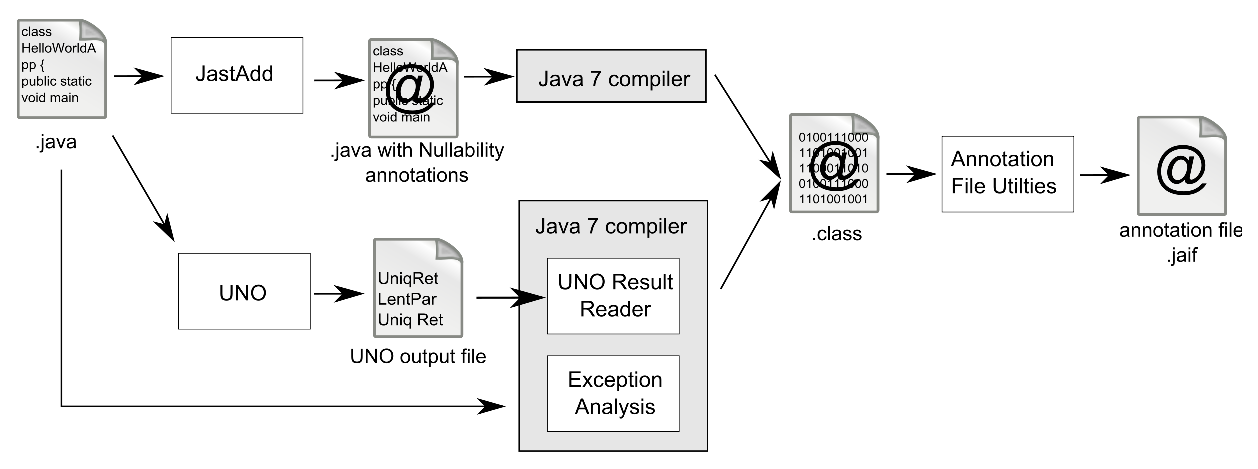
\psfig{file=figures/technicalApproach/from_source_to_jaif.eps, width=5.0in}
\caption{Toolchain from source to JAIF}
\label{fig:from_source_to_jaif}
\end{figure*}

To infer information about Java code we use three existing inference tools and 
a exception inference developed by ourselves and combine their output. 
Too aid in writing our own analyses, we have additionally developed a simple 
framework. 

To combine the results of disparate analyses we have to convert their results
into a common format.  We use the JAIF~\cite{JAIF}
(Java Annotation Index File) format for that purpose.  Some anaylses generate
results directly in JAIF format, some provide annotated bytecodes which can be
easily extracted into JAIF format, and others provide textual results for which
we will read the results into a our framework.

Figure~\ref{fig:from_source_to_jaif} 
illustrates the stages from the source to JAIF in our toolchain, explained 
below. While figure~\ref{fig:from_jaif_to_javadoc} shows how JavaGrok
puts the annotations back into the source files and generates the HTML
documentation.

\begin{figure*}
\centering
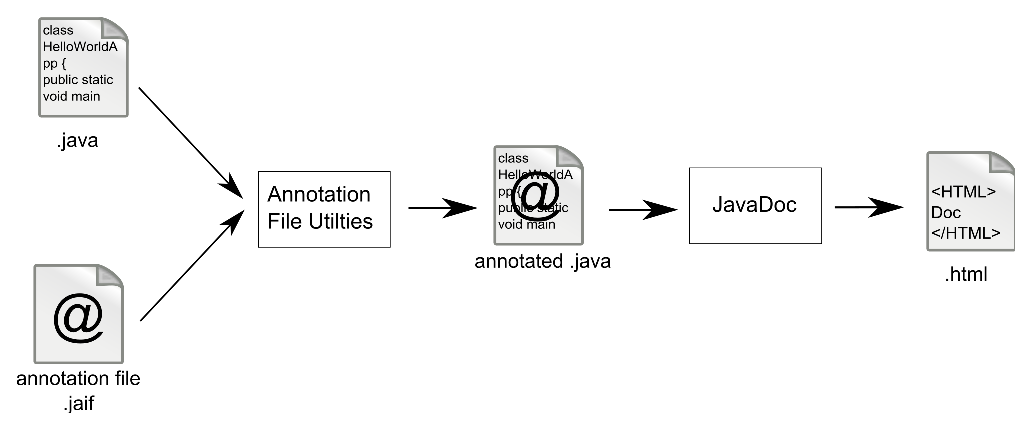
\psfig{file=figures/technicalApproach/from_jaif_to_javadoc.eps, width=5.0in}
\caption{From JAIF to Javadoc}
\label{fig:from_jaif_to_javadoc}
\end{figure*}

First Uno processes the source code which we want to annotate. 
Because Uno stores its inferred properties in a single separate file, 
we changed UNO's output format slightly.
To integrate the analysis results into the Java documentation we
use our own framework. We implemented a tree visitor inside the Java 7 
compiler that, at initialization, reads in the file generated by UNO and 
stores the information in a hashset. During the iteration over the AST
our visitor inserts annotation at the appropriate places. These then
get extracted into files in the JAIF format.

To infer exception annotation we use the Annotation Processing Tool (APT)
API~\cite{apt} built into the Java standard compiler.
% TODO: We will likely switch to also use the Type Annotation Processor! But not
% yet
From within an APT plugin
we can access the compiler's abstract syntax tree and augment the generated
bytecode with annotations representing our analysis results. These annotations
are then extracted into external annotation files.

Javarifier produces its results directly in the JAIF format which allows us to
easily integrate it into our toolchain. We need simply to express the meaning
of its inferred constraints in the Javadoc documentation in concise language.

Once the results of the various analyses have been collected into a set of
annotation files, we use the annotation file utilities~\cite{AFU} to merge
those annotations back into the original library source. This source
can now be used either directly by looking at the annotated source code. We
focus on running Javadoc over the annotated source code to generate HTML documentation
which now include our annotations.
